\documentclass[11pt]{article}
\usepackage{listings}
\usepackage{graphicx}

\begin{document}
\lstset{language=Matlab}

\title{COMPM012 - Coursework 1}
\author{Esben A. S\o rig}

\maketitle

\section{Gradient Descent Visualisation}
\begin{itemize}
    \item[a)] To produce the plot the following commands are used:
        \begin{lstlisting}
>> [X,Y] = meshgrid(linspace(0,5,15),linspace(0,5,15));
>> mesh(X,Y,fcarg(X,Y));
        \end{lstlisting}
    
        \par Which gives us the plot
        \begin{center}
        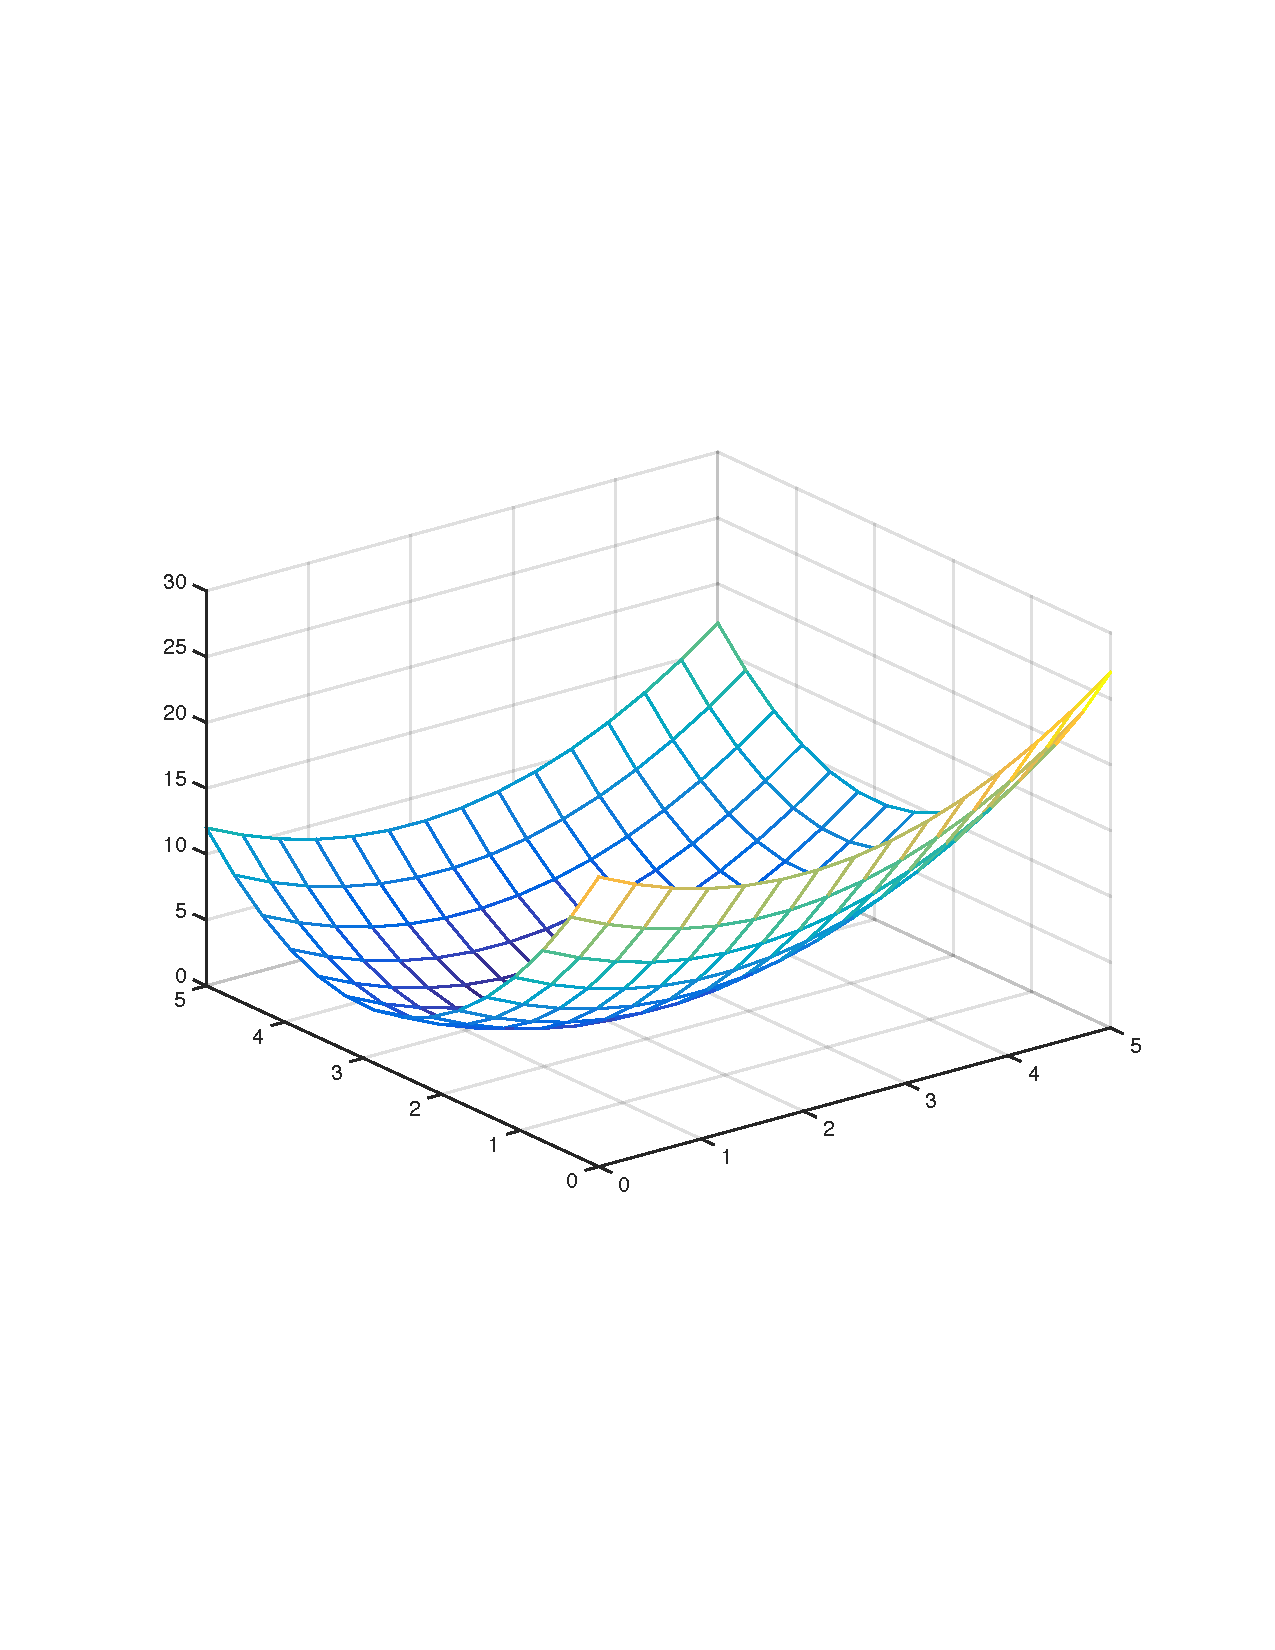
\includegraphics[width=\linewidth]{1a}
        \end{center}
    
    \item[b)]
        \begin{itemize}
        \item[i)]
            The modified graddesc function becomes:
            \begin{lstlisting}
function [soln, X, Y, Z] = graddesc(f, g, i,e, t)
    gi = feval(g,i) ;
    X = [];
    Y = [];
    Z = [];
    while(norm(gi)>t)  % crude termination condition
        i = i - e .* feval(g,i) ;
        gi = feval(g,i);
        X = [X i(1)];
        Y = [Y i(2)];
        Z = [Z fc(i)];
    end
    soln = i ;
end
            \end{lstlisting}
        
        \item[ii)]
            We produce the plot with the commands
            \begin{lstlisting}
% Gradient descent
[result, X, Y, Z] = graddesc('fc','dfc',[0,0],0.001,0.1);

% Plot descent path
hold on
plot3(X, Y, Z)
grid on
hold off
            \end{lstlisting}
            
            The obtained plot looks like
            \begin{center}
            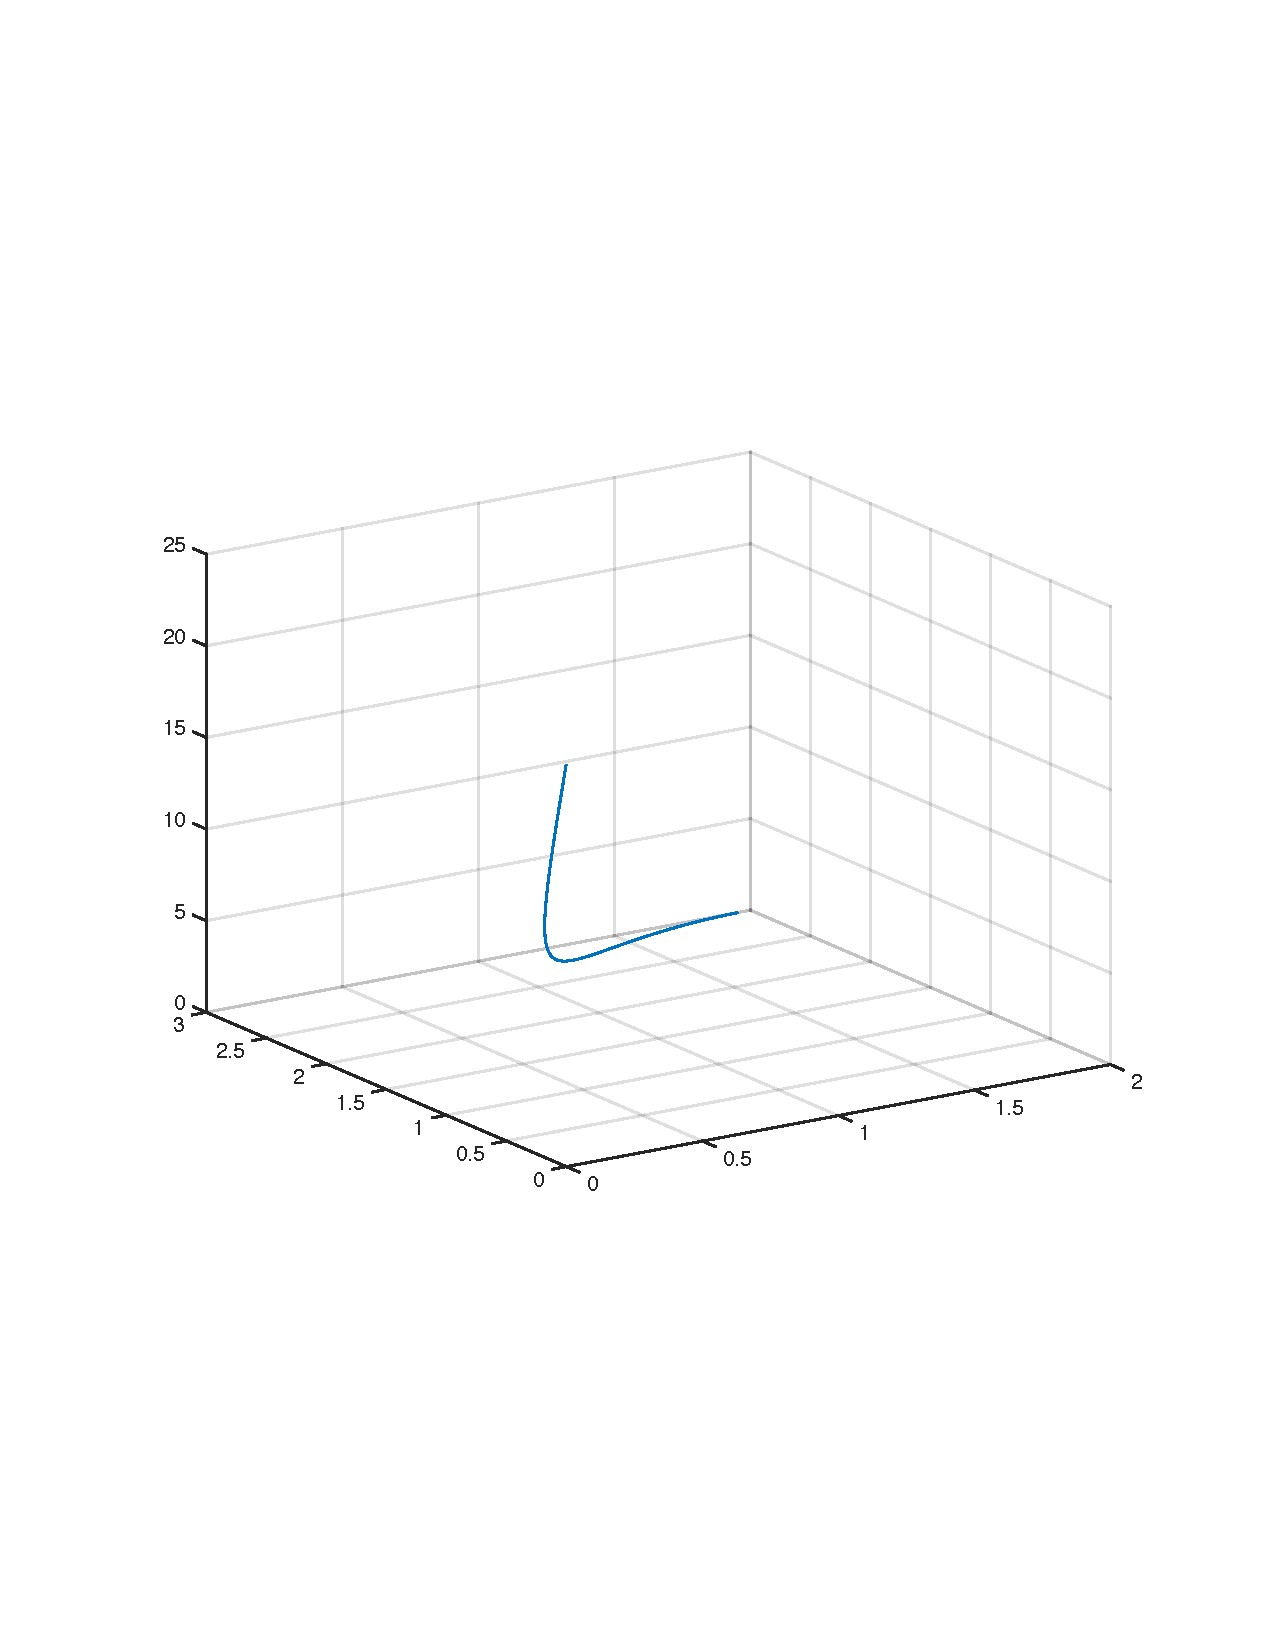
\includegraphics[width=\linewidth]{1bii}
            \end{center}
            
        \item[iii)]
            We can plot the projection to the XY-plane by simply plotting the X, Y values and ignore the Z values. We do this with the following commands
            \begin{lstlisting}
% Plot projection to XY plane
plot(X, Y)
            \end{lstlisting}
            
            Which produces the following plot
            \begin{center}
            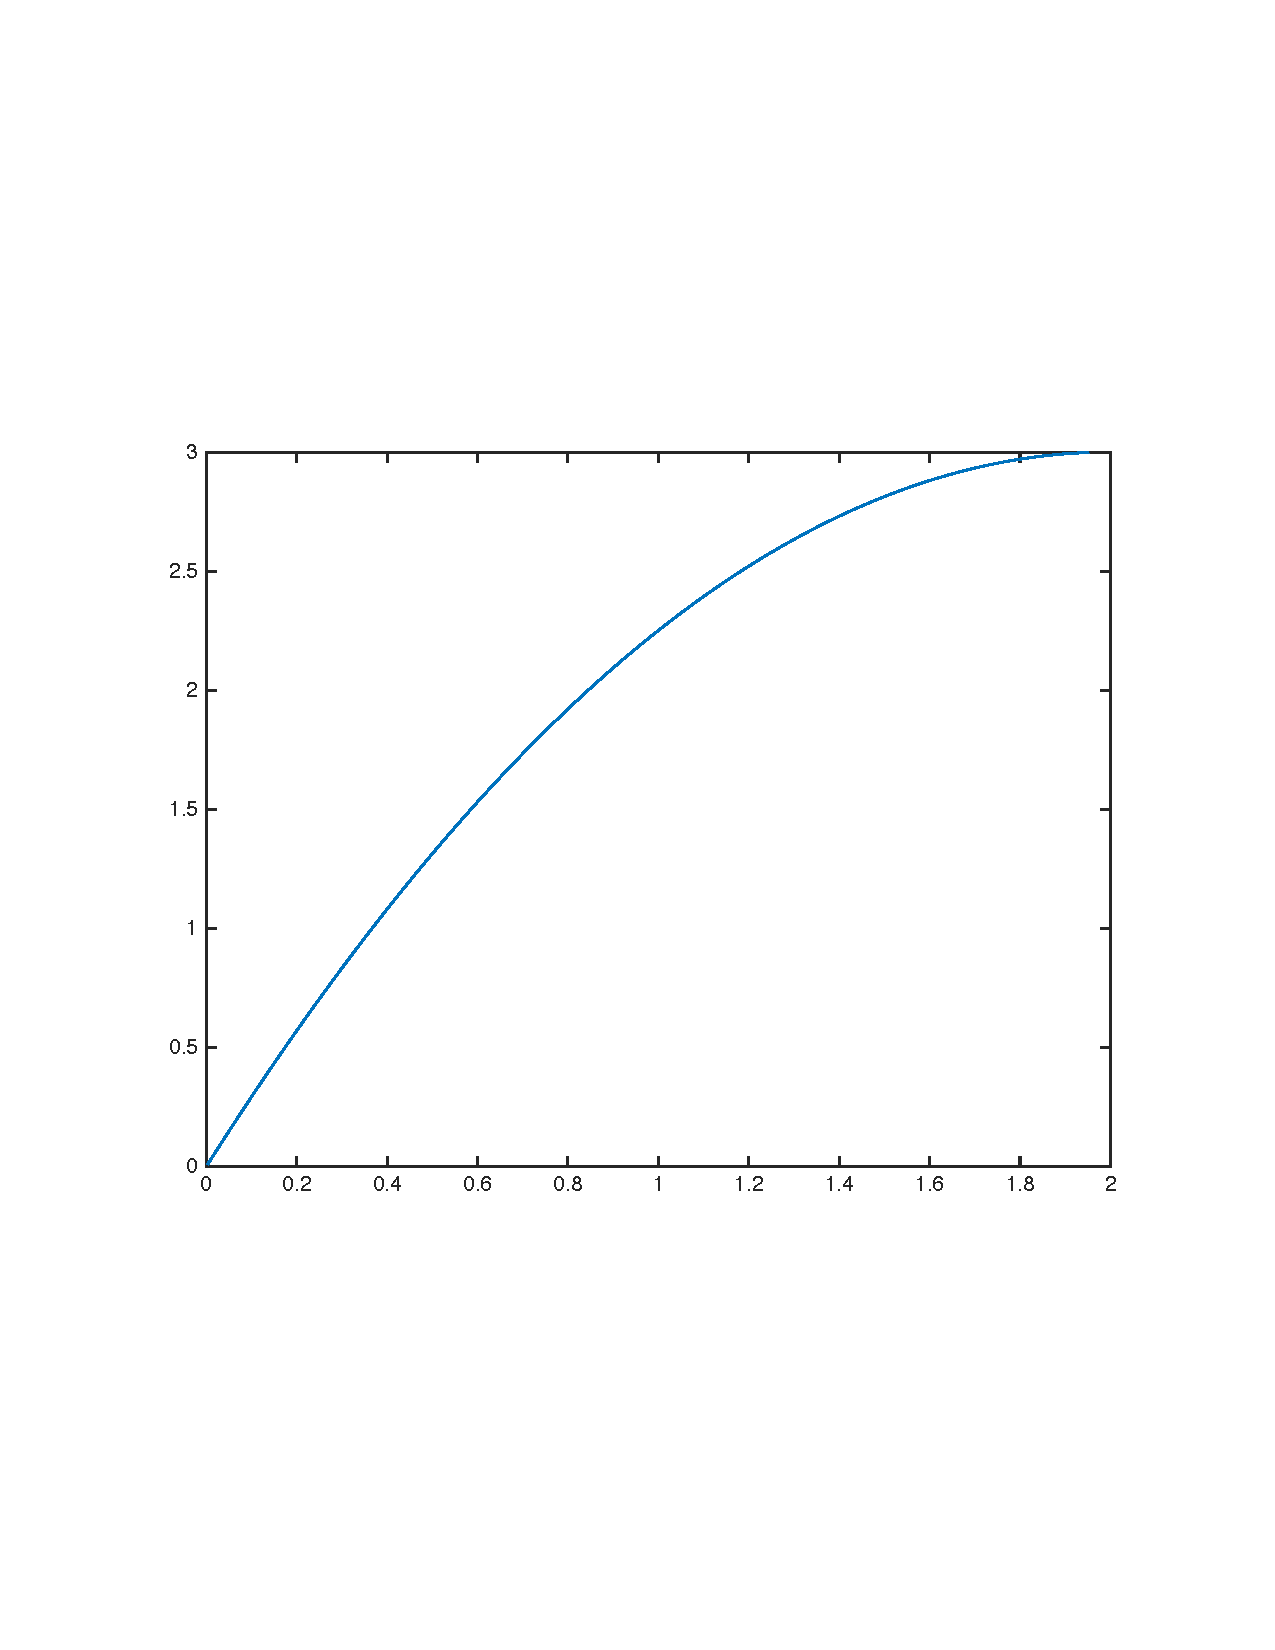
\includegraphics[width=\linewidth]{1biii}
            \end{center}
        
        \end{itemize}
        

    

\end{itemize}

\section{Gradient Descent for Linear Regression}
\begin{itemize}
    \item[a)]
        My implementation of gradient descent is
        \begin{lstlisting}
function [sol, guesses] = mygraddesc(A, b, guess, step, tol)
    mse = @(w) (A*w - b).' * (A*w - b);
    dmsedw = @(w) (-2*A.' * b) + (2*A.' * A * w);
    guesses = [guess; mse(guess)]; % Used for visualisation
    
    while norm(dmsedw(guess)) > tol
        guess = guess - dmsedw(guess)*step;
        guesses = [guesses [guess; mse(guess)]];
    end
    
    sol = guess;
end
        \end{lstlisting}
    
    \item[b)]
        We can find the solution to the system using the gradient descent implementation by putting the coefficients for $x_1$ and $x_2$ in a matrix $A$ and the right-hand-sides of the equations in a vector $b$. Passing $A$ and $b$ as arguments to the gradient descent function along with an initial guess, step size, and tolerance gives us the solution to the system. In Matlab we do:
        
        \begin{lstlisting}
A = [1 -1; 1 1; 1 2]
b = [1; 1; 3];
guess = [0; 0];

mygraddesc(A, b, guess, 0.01, 0.0001)
        \end{lstlisting}
        
        Which rerturns
        \begin{lstlisting}
ans =
    1.2857
    0.5714
        \end{lstlisting}
        
        So $x_1 = 1.2857$ and $x_2 = 0.5714$ is the least squares solution to the system.
        
    \item[c)]
        My gradient descent implementation lets us retrieve the guesses for each iteration of the descent. We plot this as follows
        \begin{lstlisting}
[~, guesses] = mygraddesc(A, b, guess, 0.01, 0.001);

plot3(guesses(1,:), guesses(2,:), guesses(3,:));
hold on
grid on
hold off
        \end{lstlisting}

        Which produces the plot
        \begin{center}
        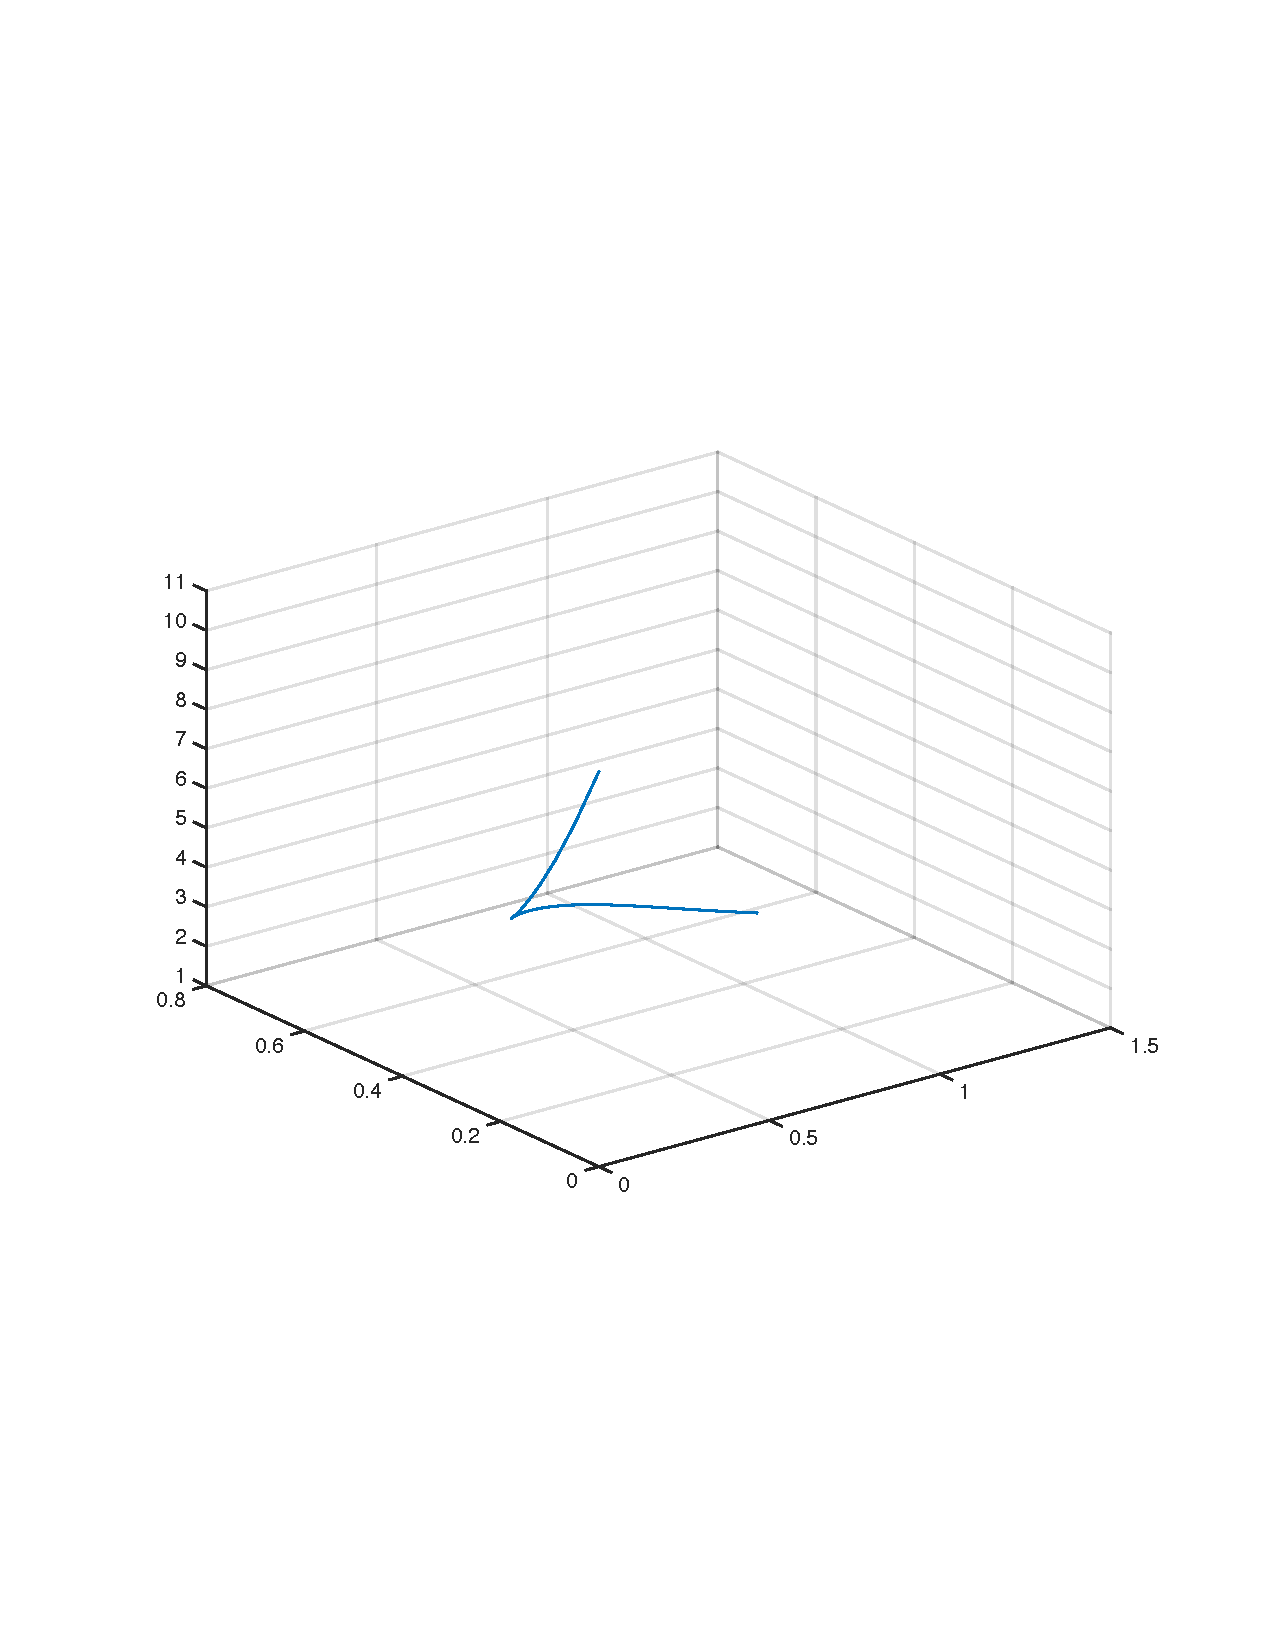
\includegraphics[width=\linewidth]{2c}
        \end{center}

\end{itemize}

\section{Convergence of Gradient Descent in a Single Variable}
\begin{itemize}
    \item[a)] We can plot the function to get an intuition.
        \begin{lstlisting}
domain = [-1:0.01:3];
range = arrayfun(@(x) abs(x-1)^3, domain);

plot(domain, range);\end{lstlisting}
        and we get
        \begin{center}
        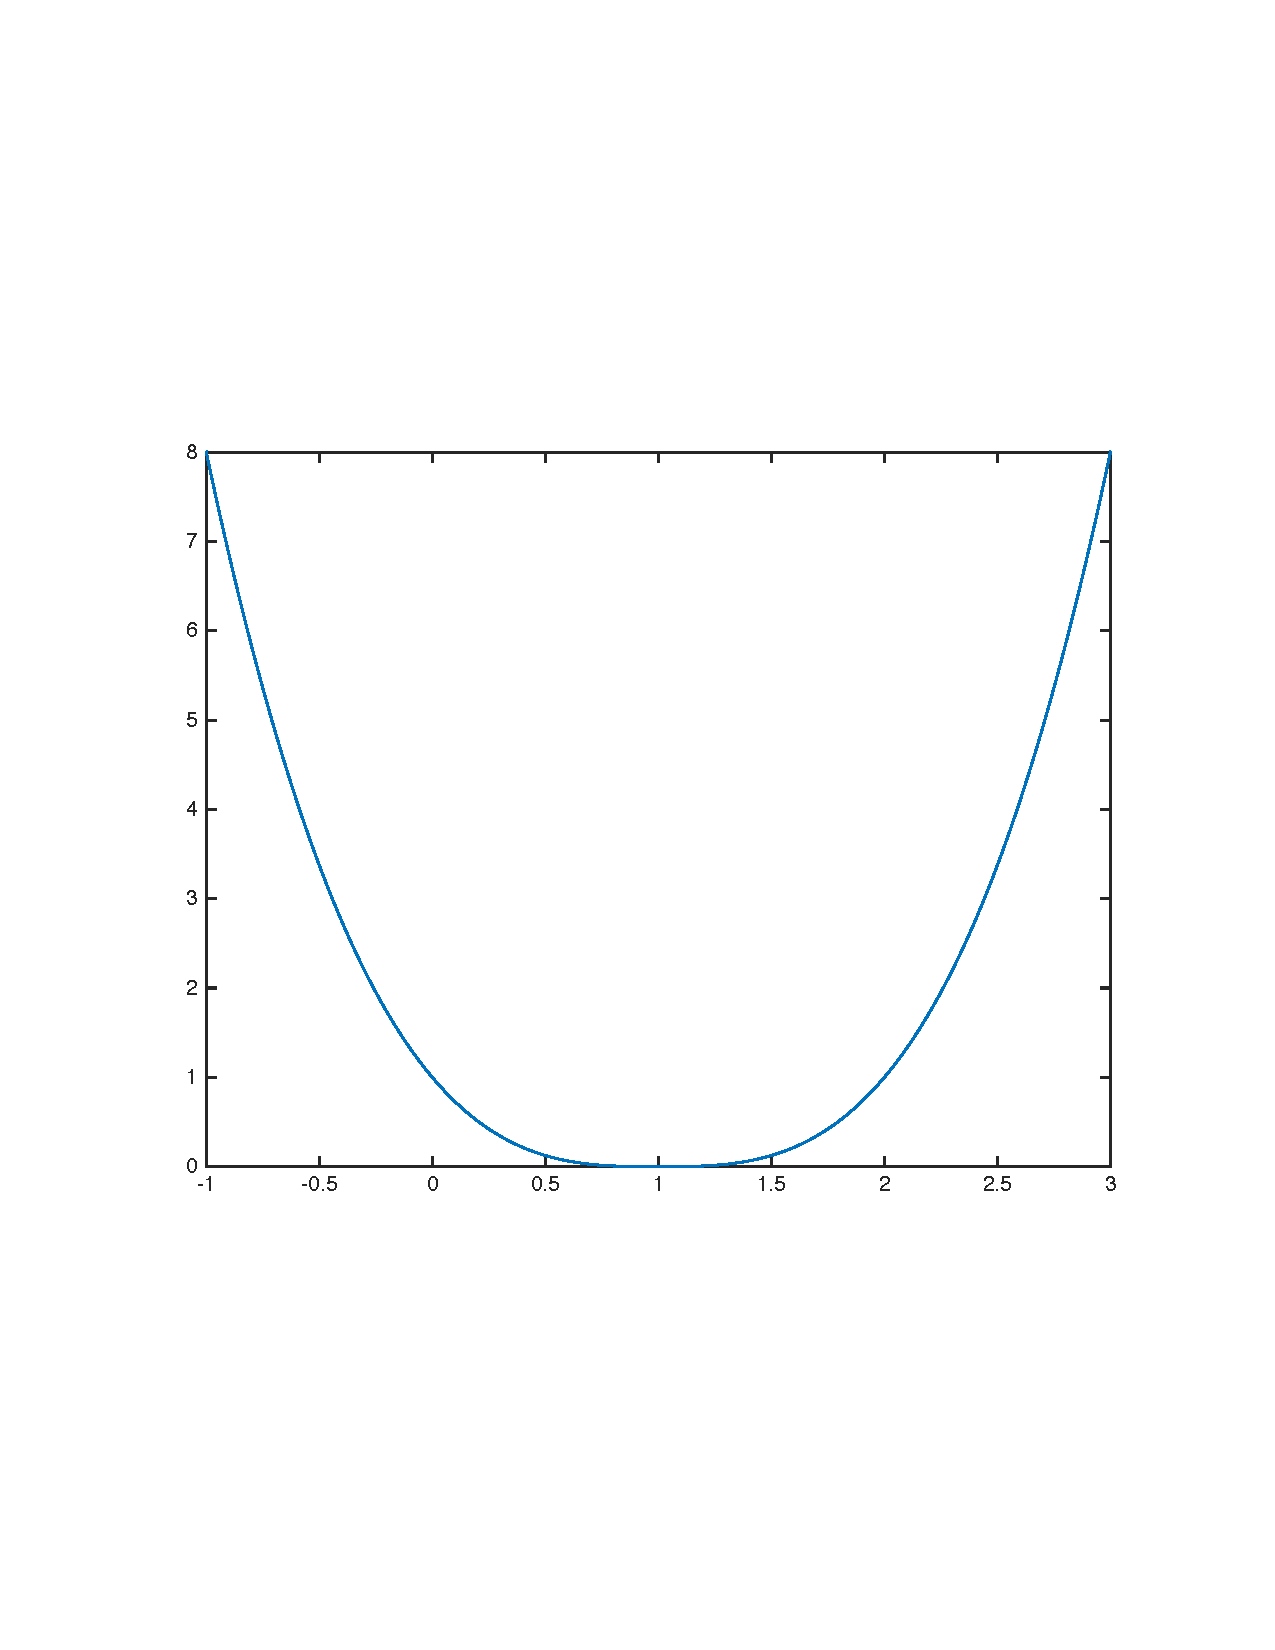
\includegraphics[width=\linewidth]{3a}
        \end{center}
        
        The function is clearly convex and gradient descent will converge for any $x_0$ and a small step size, say $\lambda = 0.01$.

    \item[b)] Again, we plot the function
    \begin{lstlisting}
domain = [-1:0.01:3];
range = arrayfun(@(x) sqrt(abs(x-1)), domain);

plot(domain, range);\end{lstlisting}
        And obtain
        \begin{center}
        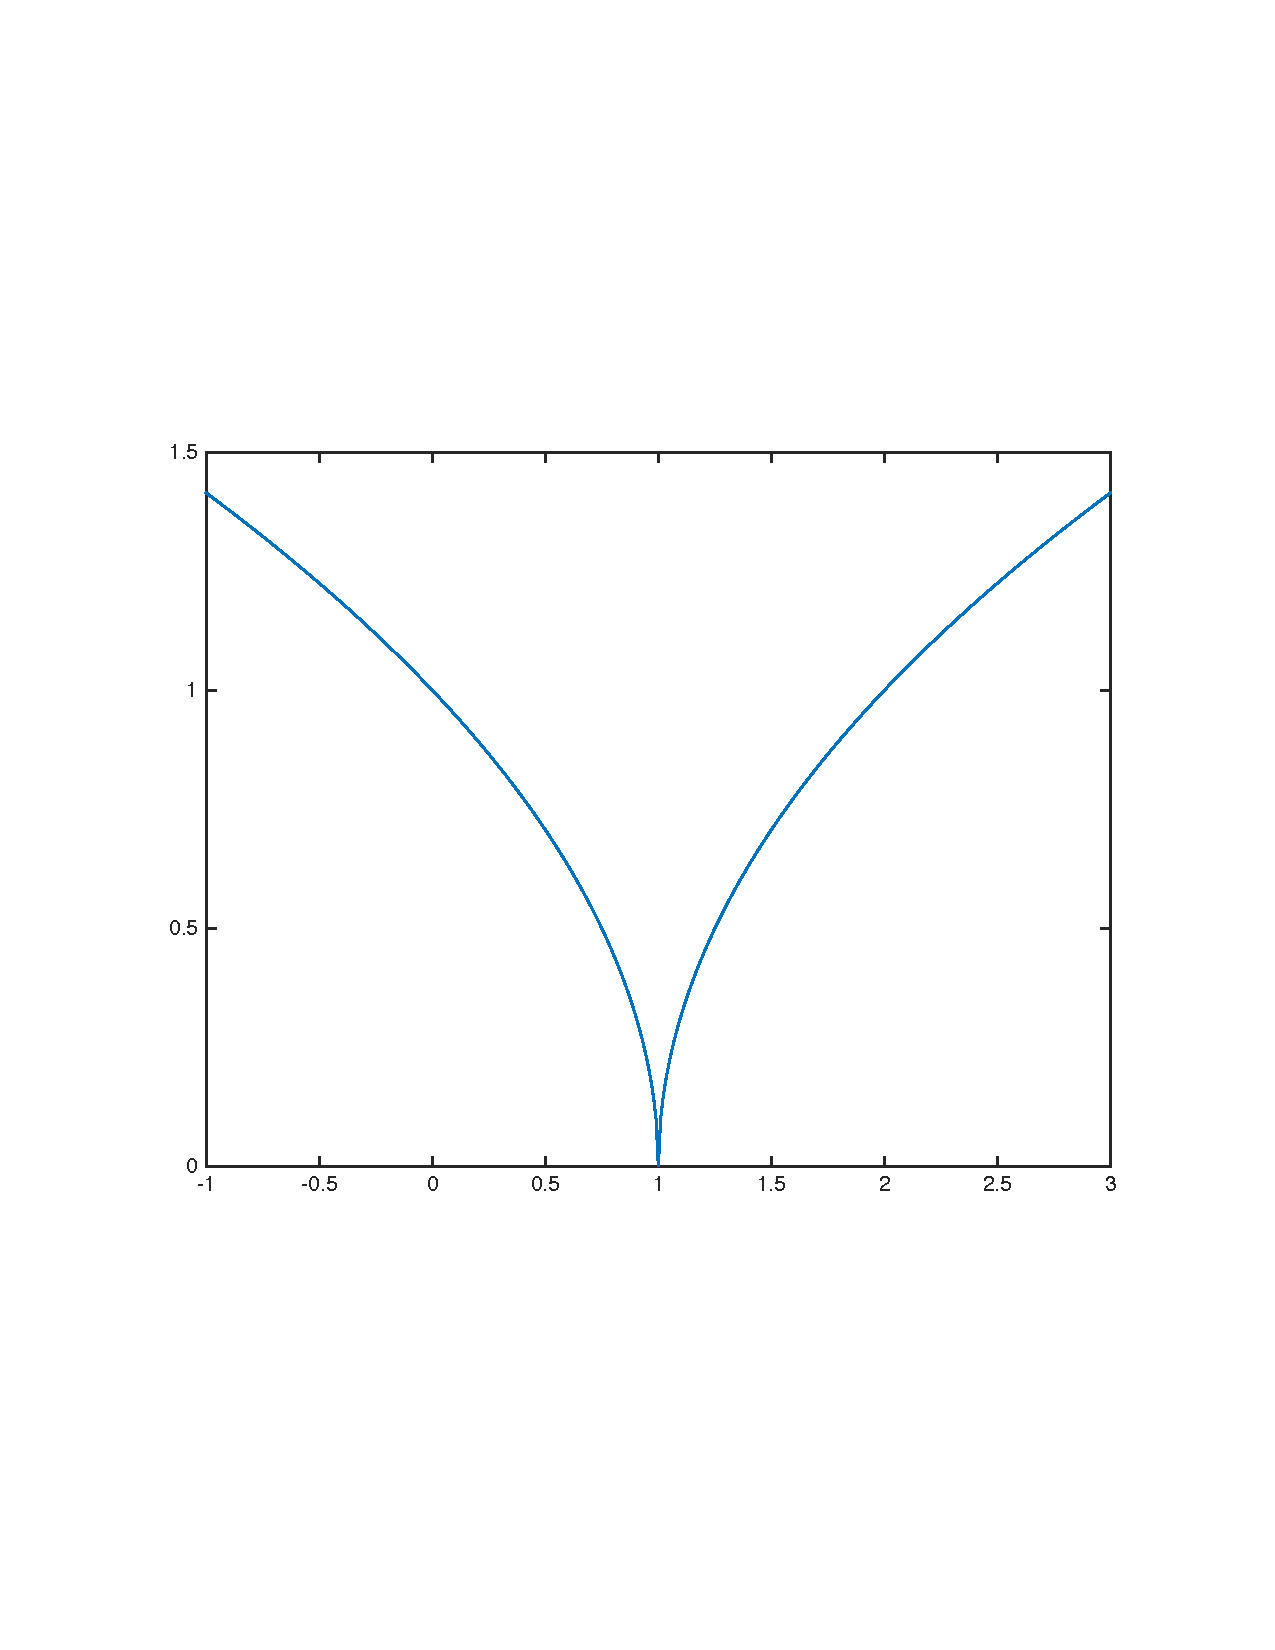
\includegraphics[width=\linewidth]{3b}
        \end{center}
        
        This function is clearly not convex and gradient descent will not converge for any $x_0$ and $\lambda$ unless $x_0 = 1$.
    
    
    \item[c)] $x^4 + 5x^2$ is a convex function with one minimum. We can show this by observing that $x^4$ is convex and $x^2$ is convex and $x^4 + 5x^2$ is therefore a convex combination of two convex functions. Therefore gradient descent will converge.
\end{itemize}


\end{document}
